\documentclass[11pt]{article}

% --------------------------
% Packages
% --------------------------
\usepackage[utf8]{inputenc}
\usepackage[T1]{fontenc}
\usepackage{lmodern}              % Better font
\usepackage{geometry}             % Adjust page margins
\geometry{margin=1in}
\usepackage{graphicx}             % For images
\usepackage{caption}              % For custom captions
\usepackage{subcaption}          % For subfigures
\usepackage{amsmath, amssymb}     % Math symbols
\usepackage{booktabs}             % Better tables
\usepackage{hyperref}             % Clickable references
\usepackage{enumitem}             % Customizable lists
\usepackage{xcolor}               % Colors
\usepackage{float}                % Force figure placement
\usepackage{authblk}              % For author affiliations
\usepackage{natbib}
%% \renewcommand{\includegraphics}[2][]{}
% --------------------------
% Title and Authors
% --------------------------
%\title{Inferring gene co-expression networks from scRNA-seq data using partial correlation coefficients}
\title{Efficient Inference of Direct Gene–Gene Associations via High-Dimensional Precision Matrix with Rigorous FDR Control}

\author[1,$\dagger$]{Feifei Ran}
\author[2,$\dagger$]{Jing Li}
\author[1]{Ying Liu}
\author[1]{Bin Lian}
\author[3,$\ast$]{Jie He}
\author[1,$\ast$]{Jialu Hu}

\affil[1]{School of Computer Science, Northwestern Polytechnical University, 1 Dong Xiang Rd., 710129, Shaanxi, China. Tel: 029-88431519.}
\affil[2]{Xi'an Mingde Institute of Technology, School of Information Engineering, 1 Mingde Rd., 710124, Shaanxi, China}
\affil[3]{School of Mathematics, Nanjing University of Aeronautics and Astronautics, 29 Jiangjunda Rd., 211106, Nanjing, China.}
\affil[$\dagger$]{These authors contributed equally.}
\affil[$\ast$]{These authors are co-responding authors.}
\date{}  
% or \date{June 2025} or leave blank for no date

% --------------------------
% Document
% --------------------------
\begin{document}
\maketitle

\begin{abstract}
Gene coexpression networks (GCNs) represent complex patterns of coordinated gene activity by modeling pairwise relationships between genes.
Reconstructing GCNs from single-cell transcriptomic data is essential for the identification of gene modules, the inferring of cell-type-specific regulatory programs, and the exploration of dynamic transcriptional changes in diverse cellular states and developmental trajectories.
However, predicting gene coexpression networks remains challenging due to confounding effects and the low inference accuracy of the graph structure under the high dimensional settings. 
We propose a novel method, dGGAPM (Direct Gene-Gene Associations via Precision Matrix), which reconstructs gene coexpression networks by statistically inferring direct gene-gene relationships. Unlike conventional approaches that rely on pairwise correlation measures and may capture indirect associations, dGGAPM leverages precision matrix to more accurately characterize the graph structure with direct interactions between genes by controlling for the influence of all other genes. The main contributions of this research are threefold. First, in contrast to existing methods, we construct the high-dimensional gene network using an estimated precision matrix, providing a rigorous and principled foundation for statistical inference of gene–gene relationships. Second, we recover the network structure through a high-dimensional multiple testing procedure that takes advantage of the asymptotic properties of the precision matrix estimator. Finally, we introduce a data-driven thresholding strategy that achieves strict false discovery rate (FDR) control, ensuring reliable identification of coexpression links in high-dimensional settings. The dGGAPM can also be used to identify functionally coherent gene modules and gain insight into their regulatory relationships. Although some nonlinear models can capture more complicated correlation relationships, a rigorous statistical inference method is challenging compared to the proposed dGGAPM.
We evaluated dGGAPM on multiple publicly available single-cell transcriptomic datasets and benchmarked its performance against several state-of-the-art network inference algorithms.  
The results demonstrate that dGGAPM consistently achieves superior performance in terms of precision, specificity, and biological relevance, highlighting its potential as a robust tool for gene network reconstruction and functional module analysis.
The source code of the dGGAPM is freely available at \href{https://github.com/jhu99/dGGAPM}{https://github.com/jhu99/DGGAPM}.
\end{abstract}

\newpage
\section*{Introduction}
Gene coexpression networks (GCNs) can be leveraged to predict cell-type-specific transcriptional states and uncover a wide range of underlying biological processes in single-cell RNA sequencing (scRNA-seq) data \citep{review,hecker2009gene}. 
In these networks, nodes correspond to genes, while edges indicate interactions relationships among genes, typically inferred through correlation or mutual information measures \citep{specht2015estimation, albert2002statistical}. 
By capturing coordinated gene activity patterns, GCNs enable the identification of regulatory modules, inference of gene functions, and characterization of cell identity and heterogeneity across diverse cellular contexts.
GCNs are also widely utilized to infer functions of previously uncharacterized genes by leveraging the known functions of co-expressed genes and their regulatory relationships \citep{parsana2019addressing}.
Through further analysis of network modules, more advanced tasks can be accomplished, including the identification of core genes within modules, association of gene modules with phenotypic traits, and modeling of metabolic and signaling pathways \citep{langfelder2008wgcna}.
Thus, accurate estimation of coexpression relationships between genes is essential for reliable inference of gene coexpression networks. 
Recent studies have utilized functional networks derived from scRNA-seq data to address key biological questions, shedding light on transcriptional regulatory mechanisms in various contexts, including cancer progression \citep{zhang2021single}, immune system response \citep{wen2020immune}, and embryonic development \citep{shangguan2020application}. 
However, current single-cell RNA sequencing (scRNA-seq) technologies are subject to several technical limitations that can introduce substantial artifacts into downstream analyzes. First, scRNA-seq data are characterized by a high prevalence of zero counts—commonly referred to as “dropouts”—and relatively inaccurate low expression counts, which arise from a combination of technical noise and intrinsic biological variability \citep{kharchenko2014bayesian, li2018accurate, azizi2017bayesian}. These artifacts can obscure true gene expression signals and distort inferred relationships. Second, variability in the depth of cell-specific sequencing—often caused by uneven loading of single-cell libraries into sequencing reactions—leads to inconsistent data quality. Third, the dynamic range of gene expression in single-cell datasets is typically compressed relative to bulk RNA-seq data, placing demands on the robustness and sensitivity of correlation-based inference methods. 

Pearson correlation and Spearman correlation are often used to infer gene coexpression networks because of their computational efficiency and strong statistical properties.
However, a significant drawback is that Pearson and Spearman correlations primarily focus on specific gene pairs during analysis. In reality, the correlation patterns within gene expression data are often intricate, influenced by numerous unmeasurable confounders. Consequently, analyzes based solely on these metrics can produce unconvincing results unless spurious inferences are adequately filtered out \citep{partial}.
To solve these problems, several computational approaches have been 
proposed, such as scLink \citep{scLink}, SCODE \citep{SCODE}, GENIE3 \citep{GENIE3,greenfield2010dream4} etc, in the last two decade.
ScLink is a method that adapts the Gaussian graphical model to infer gene coexpression networks. 
SCODE focuses on differentiated cells by integrating the transformation of linear ordinary differential equations (ODEs) with linear regression.
It takes into account the temporal aspect of each cell when assessing 
regulatory relationships between genes.
GENIE3 decomposes the task of inferring a gene regulatory network from bulk RNA-seq data among p genes into p individual regression problems, using tree-based ensemble methods to predict regulatory relationships and assign edge weights.
It has also been integrated into an SCENIC framework \citep{aibar2017scenic} for network inference from scRNA-seq data.
Later, GRNBoost2 \cite{moerman2019grnboost2} is proposed to solve the problem of GCN inference using Gradient Boosting Machine (GBM) regression and the GENIE3 framework.
However, their reliance on strong assumptions and limited capacity to capture indirect interactions or complex, non-linear dependencies may reduce their effectiveness in modeling intricate single-cell gene expression patterns.

These challenges highlight the need for analytical approaches that are capable of accommodating data sparsity, heterogeneity, and signal compression while preserving biologically meaningful coexpression patterns.
To address the challenges, we propose a novel method, dGGAPM, which recovers the gene coexpression networks by statistical inference on the  precision matrix with a FDR controlled threshold for single-cell RNA sequencing (scRNA-seq) data \citep{partial}. 
In contrast to many existing approaches that rely on conventional correlation measures that capture only pairwise associations, precision matrix quantifies the direct linear relationship between two variables while conditioning on the influence of all other variables. This adjustment allows dGGAPM to effectively account for hidden or unmeasured confounding factors, thereby yielding a more accurate representation of gene-gene dependencies. By removing the indirect effects of the intervening variables, precision matrix offers a closer approximation to the true regulatory relationships embedded in gene expression data. 
In summary, we provide a more robust and biologically interpretable framework compared to existing methods, establishing a solid foundation for downstream analyzes and advancing our understanding of cellular function and regulation in the life sciences.

\section*{Results}
\subsection*{Methods overview}
Here, considering the problem of reconstructing gene coexpression network, we propose a novel method, dGGAPM (Direct Gene–Gene Associations via
High-Dimensional Precision Matrix) by statistically inferring direct correlation relationships among genes.
As shown in \hyperref[fig:overview]{Fig. \ref{fig:overview}}, it takes a normalized expression matrix as input and uses a sparse Lasso-based scaled linear regression to estimate the precision matrix of genes, along with an adaptive thresholding strategy, thus facilitating the construction of gene coexpression networks (GCNs) from sparse scRNA-seq data while effectively removing the influence of confounding factors.
We evaluated the effectiveness and accuracy of dGGAPM by benchmarking it against several state-of-the-art algorithms using three real-world single-cell transcriptomic datasets.
The correlation relationships estimated by dGGAPM were further employed in a variety of downstream analyzes, including the identification of functional modules, gene set enrichment analysis, and the exploration of cell type-specific coexpression patterns. 
These applications underscore the versatility and biological relevance of dGGAPM in extracting structured insights from high-dimensional and noisy single-cell RNA-seq data.
The source code used in this study is freely accessible at \href{https://github.com/jhu99/dGGAPM}{https://github.com/jhu99/dGGAPM}.

\subsection*{Identification of gene coexpression networks from human embryonic stem cells}

To assess the efficiency of dGGAPM in capturing dynamic gene expression changes, we applied our algorithm alongside four widely used methods, including scLink, GENIE3, SCODE, and GRNBoost2, to a time-course single-cell RNA-seq dataset comprising 758 cells collected during the differentiation of human embryonic stem cells (hESCs) into definitive endoderm cells \citep{hESC}. This dataset includes gene expression profiles measured at six distinct time points—0, 12, 24, 36, 72, and 96 hours—thereby capturing the temporal transcriptional dynamics underlying early developmental processes. After that, we quantitatively evaluated the performance of each method using several established metrics, including the area under the receiver operating characteristic curve (AUROC), area under the precision-recall curve (AUPRC), and biological pathway enrichment of the inferred gene modules. 

As shown in \hyperref[fig:hESC1]{Fig. \ref{fig:hESC1}a}, we succesfully identified five clusters of genes from a correlation matrix calculated by dGGAPM.
Each red dot in the figure represents positive correlations and purple represents negative correlations.
To further elucidate the specific roles of the five gene clusters identified through dGGAPM, we conducted gene-set enrichment analysis. 
We selected the top six pathways of each gene set and ploted them into a heatmap as shown in (\hyperref[fig:hESC1]{Fig. \ref{fig:hESC1}b}).
Genes grouped in Cluster 1 are predominantly associated with cell differentiation processes critical for kidney development. Cluster 2 comprises genes primarily involved in endodermal cell fate commitment and DNA biosynthetic processes. Genes in Cluster 3 are enriched for pathways regulating glucose homeostasis and the positive regulation of macroautophagy. Cluster 4 includes genes that play a central role in the differentiation of natural killer T (NK T) cells, while Cluster 5 contains genes implicated in cartilage morphogenesis.
Results demonstrate that each gene cluster is involved in distinct biological processes during cell differentiation, which further validates the rationality of the gene correlation relationship and clustering results obtained through dGGAPM.

Next, we reconstructed gene coexpression networks by retaining only those edges that passed false discovery rate correction (FDR < 0.05). As shown in \hyperref[fig:hESC1]{Fig. \ref{fig:hESC1}c}, each vertex in the network represents a gene, color-coded according to its assigned cluster. Edges denote gene–gene interactions, with red indicating positive correlations and gray indicating negative correlations. The thickness of each edge reflects the interaction strength, represented by the absolute value of the correlation coefficient.
Based on the results from the enrichment analysis, we identified several gene modules within the coexpression network, each of which plays a crucial role in specific biological processes. Specifically, the results show that:
\begin{itemize}
\item The module consisting of TFAP2A, NOTCH2, and STAT1 genes is primarily involved in kidney development \citep{takasato2014directing}, contributing to the formation and functional maturation of kidney structures,
\item NANOG and SOX2 are key in the commitment of endodermal cell fate \citep{jaremko2013regulation}, regulating the differentiation and specification of the endoderm during early embryonic development,
\item PCNA, KAT7, and DTL are pivotal in DNA biosynthesis, ensuring the accurate replication and transmission of genetic information,
\item PRDM1 and ITPR1 play significant roles in late embryonic development \citep{palli2021epigenetic}, impacting the maturation and functionality of various tissues and organs,
\item HAND2 and RSPO2 are associated with cartilage development \citep{quintana2009morphogenetic}, influencing the formation and morphological transformation of cartilage tissues through gene expression regulation and signaling pathways.
\end{itemize}
These findings provide potential drug targets for research on kidney development, embryonic stem cell differentiation, DNA replication, and chondrogenesis. 

To evaluate the performance of dGGAPM, we used two metrics—ROC curve analysis and the number of true positive edges—to comprehensively evaluate the performance of our proposed method against four existing methods: scLink, GENIE3, SCODE, and GRNBoost2.
Through ROC curve analysis, our method demonstrated superior performance with an Area Under the Curve (AUC) of $0.7917$, significantly higher than scLink ($0.5947$), GENIE3 ($0.6119$), SCODE ($0.5519$), and GRNBoost2 ($0.5689$) (\hyperref[fig:hESC2]{Fig. \ref{fig:hESC2}a}). 
To assess sensitivity, we quantified the number of true‐positive edges among the top 1,000 ranked edges derived from a subset of 100 genes. As shown in \hyperref[fig:hESC2]{Fig.~\ref{fig:hESC2}b}, our dGGAPM method identified 79 correct edges, compared with 53 for scLink, 81 for GENIE3, 62 for SCODE, and 72 for GRNBoost2. Although dGGAPM and GENIE3 recovered a similar total number of true‐positive edges, dGGAPM demonstrated superior ability to capture highly correlated interactions, outperforming the other methods on this metric.

In the reconstructed gene coexpression network, the NANOG gene exhibits close connections with multiple other genes, indicating its central position within the network. This centrality suggests that NANOG may coordinate multiple biological processes and influence the differentiation potential of human embryonic stem cells (hESCs).
We then focused on the NANOG gene within the dataset. Seven additional genes associated with NANOG were extracted from the gene coexpression network (\hyperref[fig:hESC2]{Fig. \ref{fig:hESC2}c}), and a thorough analysis was conducted on these eight genes. Considering the correlation between cells and time in the hESC data, we calculated the average expression levels of these genes at each time point (\hyperref[fig:hESC2]{Fig. \ref{fig:hESC2}d}). The line graph reveals that the expression level of NANOG gradually decreases as cell differentiation progresses, whereas the PRDM1 gene shows a negatively regulated relationship with NANOG over time. Other genes exhibited similar expression trends to NANOG, consistent with the inter-gene regulatory relationships shown in \hyperref[fig:hESC2]{Fig. \ref{fig:hESC2}c}.
We performed enrichment analyzes for these eight genes and presented the results for the top $20$ pathways in biological processes (\hyperref[fig:hESC2]{Fig. \ref{fig:hESC2}e}). For biological processes, we further refined the association between these genes and the top $10$ most significant pathways (adjusted p-value < $8.3$e-$03$), presenting them in bar charts (\hyperref[fig:hESC2]{Fig. \ref{fig:hESC2}f}).
Our analysis indicated that NANOG and SOX2 continue to play central roles during endodermal differentiation. This finding aligns with the study by \cite{nanog}, which demonstrated that genes like NANOG and SOX2 act synergistically to co-regulate a set of target genes essential for embryonic stem cell pluripotency. Specifically, NANOG plays a key role in regulating the cell fate of the pluripotent inner cell mass (ICM), maintaining the pluripotent ectodermal state, and preventing differentiation into the primitive endoderm. 
Finally, to thoroughly validate the effectiveness of dGGAPM across different gene quantities, we conducted a more comprehensive validation. Specifically, we selected the top $200$ and top $400$ high-variance genes, ranked by degree, from the ground-truth network, as well as the top $400$ genes based on degree ranking, to infer the gene coexpression network and calculate the ROC. As shown in \hyperref[fig:hESC2]{Fig. \ref{fig:hESC2}g}, dGGAPM obtained the highest AUC (0.5528), followed by SCODE (0.5155), GRNBoost2 (0.5129), GENIE3 (0.5075), scLink (0.5066).
Overall, it can be concluded that dGGAPM demonstrated superior performance in capturing gene-gene interactions from dynamic gene expression changes in human embryonic stem cells.

\subsection*{Identification of gene coexpression networks from mouse embryonic stem cells}

To validate the effectiveness and robustness of our proposed method across species, we employed an additional dataset comprising mouse embryonic stem cell (mESC) data. This dataset contains scRNA-seq expression measurements from 421 primitive endoderm (PrE) cells differentiated from mESCs, collected at five distinct time points ($0$, $12$, $24$, $48$, and $72$ hours). To evaluate the performance of our approach, we selected the top 100 highly connected genes for in-depth analysis. Initially, we extracted gene expression data for these 100 genes across the 421 cells and computed the precision matrix using our method (see Equation \ref{3}). Based on the estimated correlation coefficients, we applied the K-Means algorithm to cluster the genes into four distinct categories, containing 38, 25, 18, and 19 genes, respectively. The resulting correlation heatmap (\hyperref[fig:s1]{Fig. \ref{fig:s1}a}) illustrates positive correlations in red and negative correlations in purple. Notably, genes within the same category exhibited high correlation, whereas correlations between genes from different categories were relatively low. This pattern indicates strong intra-category cohesion and weak inter-category connectivity. This visualization effectively highlights the modular structure of the gene coexpression network, providing a way for subsequent biological analyzes.

After identifying these gene sets, we performed enrichment analyzes, selecting the six most significantly enriched pathways from each category. We then calculated the negative logarithm (-log10) of the adjusted p-values for each pathway and visualized the results in a heatmap (\hyperref[fig:s1]{Fig. \ref{fig:s1}b}). The enrichment analysis revealed that different gene modules were significantly associated with various biological pathways. In particular, genes within the first and third modules appear to play key roles in maintaining stem cell populations. Additionally, the co-enrichment of the first and fourth modules in heterochromatin organization pathways suggests that genes within these modules may share overlapping functions in regulating stem cell-specific gene expression patterns.  We highlight the corresponding pathways in \hyperref[fig:s1]{Fig. \ref{fig:s1}b} for intuitive observation and analysis. A partial representation of the gene coexpression network is depicted in \hyperref[fig:s1]{Fig. \ref{fig:s1}c}. In category $1$ (red nodes), a submodule comprising five genes was identified, which, along with another five-gene submodule detected in category $3$ (yellow nodes), is implicated in mechanisms that maintain stem cell populations and cell numbers \citep{yang2022chemical}. In category $2$ (orange nodes), a tightly knit coexpression module consisting of four genes was discovered, primarily responsible for the regulation of protein stability \citep{zhang2021mk2}, a critical process to maintain cell homeostasis and normal physiological functions. Additionally, a synergistic interaction between the genes Gata4 and Sox17 was observed in the morphogenesis of the embryonic foregut \citep{chin2017morphogenesis}. Finally, in category $4$ (green nodes), a submodule composed of the genes Amdhd2 and Hexa was found to play a significant role in dynamic metabolic processes during early mammalian embryonic development \citep{zhao2023dynamic}. These discoveries not only enhance our understanding of the mechanistic roles of gene modules in specific biological pathways but also offer valuable insights for further exploration of gene interaction networks and potential therapeutic targets.

Next, we compared dGGAPM with scLink, GENIE3, SCODE, and GRNBoost2, evaluating their performance using Receiver Operating Characteristic (ROC) curves and the number of true positive edges identified among the strongest correlations. In terms of ROC curves, the area under the curve (AUC) for our method (AUC = $0.5877$) surpassed that of the other four methods: scLink ($0.5093$), GENIE3 ($0.5314$), SCODE ($0.5159$), and GRNBoost2 ($0.5305$) (\hyperref[fig:s2]{Fig. \ref{fig:s2}a}). To further assess the statistical significance of dGGAPM, we conducted DeLong’s test to compare its AUC with those of the other methods, yielding p-values of $0.0579$, $0.1158$, $0.0414$, and $0.1093$, respectively. These results suggest that dGGAPM has a comparative advantage over the alternative approaches. Regarding true positive edges, we quantified the number of correct edges among the top $100$ and $200$ edges derived from the $100$ genes. As shown in the bar chart in \hyperref[fig:s2]{Fig. \ref{fig:s2}b}, among the top $100$ edges, dGGAPM, scLink, GENIE3, SCODE, and GRNBoost2 identified $31$, $20$, $22$, $18$, and $19$ true positive edges, respectively. For the top $200$ edges, the five methods detected $54$, $34$, $44$, $31$, and $42$ true positive edges, respectively. These findings demonstrate that, on this dataset, our method outperforms the other four approaches by identifying a greater number of true positive edges.

By sorting the nodes based on various attributes such as degree, betweenness centrality, and closeness centrality, we identified several central nodes, including Dppa2, Pou5f1, Trim28, and Sox2. These central nodes may play pivotal roles in the gene network, and any abnormal expression or functional loss of these genes could lead to significant biological consequences. 
We then focused on Sox2 and its associated genes for further investigation, specifically analyzing their interactions, as shown in \hyperref[fig:s2]{Fig. \ref{fig:s2}c}, where genes are color-coded by category. Given cells in the mESC dataset that were collected at multiple time points, we calculated the average expression of these genes at each time point to observe their dynamic expression changes. As depicted in the line chart in \hyperref[fig:s2]{Fig. \ref{fig:s2}d}, the expression of Sox2 gradually decreases as cell differentiation progresses. Furthermore, Sox2 exhibits a positive regulatory relationship with four other genes in the same category over time, while the Gata4 gene, which negatively correlates with Sox2, shows an opposite expression pattern.

Then, we performed an enrichment analysis on these six genes and visualized the top 20 biological process pathways in \hyperref[fig:s2]{Fig. \ref{fig:s2}e}. We then focused on the ten most significant pathways (with an adjusted p-value < $3.7e-04$) and examined the specific roles of individual genes within these pathways. The results are shown in a bar chart in \hyperref[fig:s2]{Fig. \ref{fig:s2}f}. The analysis highlights that Sox2, Nanog, and Gata4 collectively play a critical role in the formation and development of the endoderm. Furthermore, nine of the pathways involve both Sox2 and Nanog, which aligns with findings from human embryonic stem cell datasets. This reinforces the idea that Sox2 and Nanog work synergistically as key target genes in regulating embryonic stem cell pluripotency.


\subsection*{Identification of gene coexpression networks from mouse hematopoietic stem cells}

Finally, we applied our method to mouse hematopoietic stem cell data to assess its adaptability and effectiveness across different cell types. In line with our previous analyzes, we first identified the top 100 highly variable genes with the greatest degrees in the real network. Using the expression profiles of these genes across 1,071 cells, we computed their precision matrix. We then performed K-means clustering, which grouped the genes into five categories containing 20, 6, 6, 14, and 54 genes, respectively. The correlation heatmap in \hyperref[fig:s3]{Fig. \ref{fig:s3}a} illustrates the distribution of gene correlations within and between categories. It is evident from the heatmap that genes in category 1 exhibit weak intra-category correlations and minimal associations with genes in other categories, suggesting these genes may play a reduced role in gene regulation. Next, we conducted enrichment analyzes on these gene modules. We selected the top five significantly enriched pathways for each category and visualized the negative logarithm of the adjusted p-values (-log10) for each pathway in a heatmap, as shown in \hyperref[fig:s3]{Fig. \ref{fig:s3}b}. The enrichment analysis results indicate that specific gene modules are significantly enriched in only a few corresponding biological pathways, while showing low enrichment scores (blue regions) in pathways that are strongly enriched in other modules. This confirms the precision of our method in calculating gene precision matrix and highlights its ability to identify gene sets with distinct biological functions effectively.

The partial topological structure of the gene coexpression network inferred by dGGAPM is shown in \hyperref[fig:s3]{Fig. \ref{fig:s3}c}, with the corresponding enrichment results depicted in \hyperref[fig:s3]{Fig. \ref{fig:s3}b} using color-coded frames that represent different gene categories. Notably, the inferred network excludes genes from category 1, which aligns with the prior analysis of the precision matrix. Additionally, dGGAPM identified several biologically significant gene submodules. For instance, a module from category 2, consisting of PCNA, MCM4, CDT1, and RAD51, plays a crucial role in DNA replication \citep{fortini2012plasticity}, facilitating DNA strand elongation and damage repair. Similarly, a four-gene module in category 3 (yellow nodes) is involved in chromosome segregation and spindle assembly, processes vital for cell division. Furthermore, dGGAPM detected overlapping three- and four-gene modules, including GATA2, JUN, and FOS, which positively regulate miRNA transcription and significantly contribute to hematopoiesis regulation \citep{liao2022mouse}. Finally, a three-gene submodule within category 5 was notably enriched in pathways related to the positive regulation of protein localization to telomeres, a crucial mechanism for maintaining telomere integrity and genomic stability. These findings may provide insights into the molecular mechanisms underlying disease pathogenesis. 

For the mHSC dataset, we conducted a comparative analysis of our method against the same four established methods used in previous experiments. In this evaluation, we applied two distinct gene selection strategies and computed the corresponding ROC curves. Initially, we selected 100 highly variable genes with the highest degrees in the real network for analysis. As shown in \hyperref[fig:mHSC2]{Fig. \ref{fig:mHSC2}a}, the Area Under the Curve (AUC) obtained by dGGAPM (AUC = 0.6037) surpassed that of the other four methods: scLink (0.5550), GENIE3 (0.5484), SCODE (0.5461), and GRNBoost2 (0.5524). This result indicates that our method achieves superior accuracy in identifying gene regulatory relationships, particularly when addressing highly variable genes. Subsequently, we ranked the top 100 genes based solely on degree, and once again, dGGAPM consistently outperformed the other four methods in this dataset (\hyperref[fig:mHSC2]{Fig. \ref{fig:mHSC2}b}). These findings further highlight the enhanced capability of our approach in accurately inferring gene coexpression networks.

% For the mHSC dataset, we conducted a comparative analysis of our method against the same four established methods employed in prior experiments.
% In the evaluation process, we adopted two distinct gene selection strategies and calculated the corresponding ROC curves.
% Initially, we selected $100$ highly variable genes with the highest degrees in the real network for analysis.
% As depicted in \hyperref[fig:mHSC2]{Fig. \ref{fig:mHSC2}a}, the AUC derived by dGGAPM (AUC = $0.6037$) exceeded that of the other four methods (scLink: $0.5550$, GENIE3: $0.5484$, SCODE: $0.5461$, GRNBoost2: $0.5524$).
% This outcome suggests that our method achieves superior accuracy when addressing highly variable genes, thereby more effectively discerning gene regulatory relationships.
% Subsequently, we evaluated the top $100$ genes ranked solely by degree, and dGGAPM consistently outperformed the other four methods on this dataset (\hyperref[fig:mHSC2]{Fig. \ref{fig:mHSC2}b}).
% These findings further substantiate the enhanced capability of our approach in inferring gene coexpression networks.

To evaluate the ability of each method to detect true positive edges when predicting strong gene correlations, we calculated the number of true positive edges among the top 50 and 100 most highly correlated edges derived from a set of 100 genes (\hyperref[fig:mHSC2]{Fig. \ref{fig:mHSC2}c}). Among the top 50 edges, dGGAPM, scLink, GENIE3, SCODE, and GRNBoost2 identified 7, 5, 2, 9, and 2 true positive edges, respectively. For the top 100 edges, these methods detected 15, 11, 2, 16, and 2 true positive edges, respectively. These results show that, while dGGAPM ranks slightly below SCODE in terms of detecting gene coexpression networks, it outperforms the other three methods in terms of both effectiveness and accuracy.
% To assess the capability of each method in detecting true positive edges when predicting strong gene correlations, we calculated the number of true positive edges among the $50$ and $100$ most highly correlated edges derived from a set of $100$ genes (\hyperref[fig:mHSC2]{Fig. \ref{fig:mHSC2}c}).
% Among the top $50$ edges, dGGAPM, scLink, GENIE3, SCODE, and GRNBoost2 identified $7$, $5$, $2$, $9$, and $2$ true positive edges, respectively.
% For the top $100$ edges, these methods detected $15$, $11$, $2$, $16$, and $2$ true positive edges, respectively.
% Taken together, these evaluation outcomes demonstrate that, although dGGAPM ranks below SCODE in identifying gene coexpression networks, it surpasses the other three methods in both effectiveness and accuracy.

Our analysis successfully identified several central nodes critical to the gene coexpression network, including key genes such as JUN, GATA2, and HDAC. In subsequent investigations, we specifically focused on the GATA2 gene and its associated gene set, performing an in-depth analysis of their interactions (\hyperref[fig:mHSC2]{Fig. \ref{fig:mHSC2}d}). To clearly differentiate genes across categories, we employed unique color coding. Consistent with previous studies, we conducted enrichment analysis on these seven genes and presented the top 20 biological process pathways (\hyperref[fig:mHSC2]{Fig. \ref{fig:mHSC2}e}). We further identified the ten most significant pathways (adjusted p-value < 7.9e-05), visualized in a bar chart in \hyperref[fig:mHSC2]{Fig. \ref{fig:mHSC2}f}. The results show that GATA2, JUN, and FOS consistently feature in the top ten significantly enriched pathways, primarily contributing to the positive regulation of miRNA transcription and metabolic processes—essential functions for normal cellular activity and differentiation. GATA2, a well-known transcription factor, plays a pivotal role in several biological processes, including cell proliferation, differentiation, and apoptosis. Previous research has shown that GATA2 regulates early embryonic development and works in concert with other GATA transcription factors to control the proliferation and differentiation of granulocytic, erythroid, megakaryocytic, and mast cell lineages \citep{vicente2012role}. Additionally, GATA2 is a key regulator in hematopoiesis, with its overexpression or mutation being associated with leukemogenesis, suggesting that further investigations into GATA2 could provide new insights into leukemia pathogenesis. JUN and FOS, members of the AP-1 transcription factor family, are integral to cellular stress responses, inflammation, and tumorigenesis \citep{eferl2003ap}. The persistent expression and activity of these transcription factors can profoundly affect cell survival and differentiation, influencing disease initiation and progression. Thus, understanding their roles within these pathways enhances our comprehension of the molecular mechanisms driving cellular differentiation and presents promising targets for disease treatment and prevention.

% Our analysis successfully pinpointed several central nodes critical to the network, including key genes such as JUN, GATA2, and HDANC. 
% In subsequent investigations, we specifically concentrated on the GATA2 gene and its associated gene set, performing an in-depth analysis of their interactions (\hyperref[fig:mHSC2]{Fig. \ref{fig:mHSC2}d}). 
% To distinctly differentiate genes across categories, we employed unique color coding. 
% Consistent with prior studies, we conducted enrichment analysis on these seven genes and presented the top $20$ biological process pathways (\hyperref[fig:mHSC2]{Fig. \ref{fig:mHSC2}e}). 
% Ultimately, we identified the ten most significant pathways (adjusted p-value < $7.9$e$-05$), depicted in a bar chart in \hyperref[fig:mHSC2]{Fig. \ref{fig:mHSC2}f}. 
% This visualization demonstrates that GATA2, JUN, and FOS consistently play roles in the top ten significantly enriched pathways, primarily contributing to the positive regulation of miRNA transcription and metabolic processes—functions essential for normal cellular activity and differentiation. 
% GATA2, a well-recognized transcription factor, exerts a pivotal influence across various biological processes, including cell proliferation, differentiation, and apoptosis. 
% Previous research has shown that GATA2 regulates early embryonic development, working in concert with other GATA transcription factors to govern the proliferation and differentiation of granulocytic, erythroid, megakaryocytic, and mast cell lineages \citep{vicente2012role}. 
% Furthermore, GATA2 is a key regulator in hematopoiesis, where its overexpression or mutation may be linked to leukemogenesis, suggesting that investigations into GATA2 could yield novel perspectives on leukemia pathogenesis. 
% JUN and FOS, members of the AP-1 transcription factor family, are integral to cellular stress responses, inflammation, and tumorigenesis \citep{eferl2003ap}. 
% The persistent expression and activity of these transcription factors may profoundly affect cell survival and differentiation, consequently influencing disease initiation and progression. 
% Thus, elucidating their roles within these pathways deepens our understanding of the molecular mechanisms driving cellular differentiation and offers promising targets for disease treatment and prevention. 

\section*{Methods and materials}
\subsection*{Inferring gene coexpression networks from scRNA-seq data}

To illustrate this point, consider a toy example involving a $p$-dimensional random vector 
$\mathbf{X}=(X_1,X_2,\ldots$ $,X_p)^\top$, where the goal is to recover the underlying network structure of $\mathbf{X}$ in a high dimensional setting with large $p$. A straightforward approach is to estimate the sample correlation matrix of $\mathbf{X}$, denoted by $\mathbf{\Sigma}$, where off-diagonal entry $\sigma_{ij}$ corresponds to the Pearson correlation coefficient between $X_i$ and $X_j$, for all $i\neq j\in\{1,\ldots,p\}$. However, Pearson correlation is easily influenced by multicollinearity within $\mathbf{X}$. Suppose that both $(X_1,X_2)$ and $(X_1,X_3)$ are highly correlated, while $(X_2,X_3)$ are independent. Due to the presence of both direct and indirect associations, the estimated Pearson correlation between $X_2$ and $X_3$ tends to be artificially inflated--an effect that becomes even more pronounced in high-dimensional settings. In contrast, the situation is entirely different for the precision matrix, which is the inverse of the correlation matrix. Each entry of the precision matrix, denoted by $\omega_{ij}$, corresponds to the partial correlation between $X_i$ and $X_j$, by removing the influence of all remaining variables $\mathbf{X}_{-(i,j)}=(X_k,k=1,\ldots,p,k\neq i,j)^\top$. As a result, the estimated dependence structure is much more accurate. In essence, the precision matrix improves upon marginal correlation by filtering out spurious associations induced by other related variables. It has seen widely applied across various fields. For instance, \cite{peng2009partial} introduced a nodewise regression approach to estimate the precision matrix in high-dimensional, low-sample-size scenarios. Their method consists of two main steps: first, estimating the precision matrix for high dimensional random vector by minimizing a joint sparse regression model based loss function; and second, inferring the network structure from the estimated precision matrix. Building on this foundation, \cite{qiu2020estimating} proposed a $c$-level high dimensional multiple testing procedure for precision matrix. In this framework, variable pairs whose corresponding estimated precision matrix entries exceed a predefined threshold in absolute value are connected by edges and subsequently tested for significance. This method was applied to the analysis of brain imaging data from patients with Alzheimer’s disease.


Motivated by these researches, we aim to extend the application of the statistical inference for the precision matrix to the analysis of gene coexpression networks based on single-cell data. Our research can be summarized by the following main steps:
1. Data Preprocessing.
For the human embryonic stem cell (hESC) dataset, we conducted preprocessing using the Seurat workflow. Specifically, cells with fewer than 6,000 or more than 12,000 detected genes were filtered out, along with those exhibiting a mitochondrial gene proportion exceeding 10\%. Additionally, genes expressed in fewer than 10\% of cells were removed. The data were then normalized using Seurat's default LogNormalize method. After preprocessing, the final dataset contained 13,069 genes across 714 cells. 
For the mouse embryonic stem cell (mESC) dataset, we applied a log transformation to transcripts per kilobase million (TPM) or fragments per kilobase million (FPKM) values, using a pseudo-count of 1. The transformed values were treated as gene expression levels. As with the hESC dataset, genes expressed in fewer than 10\% of the cells were filtered out. The resulting dataset included 18,385 genes across 421 cells.
For the mouse hematopoietic stem cell (HSC) dataset, we focused on erythroid lineage data obtained from three hematopoietic lineages (erythroid, granulocyte-monocyte, and lymphoid), following a previous study \citep{Beeline}. The final processed dataset consisted of 4,762 genes with standardized expression values across 1,071 cells.

2. Estimating the precision matrix.
Denote by $\mathbf{y}=(y_1,\ldots,y_p)^\top$ the population-level gene expression vector, where $p$ represents the number of genes. More specifically, let $y_{i,j}$ be the expression value of the $j$th gene in the $i$th cell, for $i=1,\ldots,n$ and $j=1,\ldots,p$, where $n$ denotes the number of cells.
By collecting all expression values of the $j$th gene across the $n$ cells, we obtain an $n$-dimensional expression vector $\mathbf{y}_j=(y_{1,j},\ldots,y_{n,j})^\top$, for $j=1,\ldots,p$.
Following the approach of \cite{peng2009partial}, 
%all entries of the precision matrix, that is the correlation between two entries of $\mathbf{y}$, can be estimated by fitting $p$ node-wise regression models, each of the form:
the precision matrix can be estimated by fitting $p$ node-wise regression models, each of the form:
\begin{equation}\label{1} 
y_j=\alpha_{j,0}+\boldsymbol{\alpha}_j^\top\mathbf{y}_{-j}+\epsilon_j
\end{equation}
for $j=1,\ldots,p$, where $\mathbf{y}_{-j}=(y_1,\ldots,y_{j-1},y_{j+1},\ldots,y_p)^\top$ denotes the $p-1$-dimensional vector obtained by removing the $j$th element from $\mathbf{y}$. The vector $\boldsymbol{\alpha}_j=(\alpha_{j,1},\ldots,\alpha_{j,p-1})^\top$ represents the regression coefficients corresponding to  $\mathbf{y}_{-j}$, and $\epsilon_j$ is the error term in the regression model (\ref{1}). 
According to the results in \citep{peng2009partial}, the regression error $\epsilon_{j_1}$ is uncorrelated with $\mathbf{y}_{-j_1}$ if and only if $\alpha_{j_1,j_2} = -\omega_{j_1,j_2}/\omega_{j_1,j_1}$ for any $j_2 \ne j_1$, where $\omega_{j_1,j_2}$ denotes the $(j_1,j_2)$-th element of the precision matrix.  Let $v_{j_1,j_2}$ denote the sample covariance between regression errors $\epsilon_{j_1}$ and $\epsilon_{j_2}$, which can be estimated by
\begin{equation}\label{2}
    \hat{v}_{j_1,j_2}=\begin{cases}
        -\dfrac{1}{n}\sum\limits_{i=1}^n(\hat{\epsilon}_{i,j_1}\hat{\epsilon}_{i,j_2}+\hat{\alpha}_{j_1,j_2}\hat{\epsilon}_{i,j_2}^2+\hat{\alpha}_{j_2,j_1}\hat{\epsilon}_{i,j_1}^2) &, j_1\ne j_2,\\
        \dfrac{1}{n}\sum\limits_{i=1}^n\hat{\epsilon}_{i,j_1}\hat{\epsilon}_{i,j_2} &, j_1=j_2.
    \end{cases}
\end{equation}
Denote $\rho_{j_1,j_2}$ as the partial correlation between genes $y_{j_1}$ and $y_{j_2}$. 
From equation (\ref{2}), we can derive the estimation of $\rho_{j_1,j_2}$ as following
\begin{equation}\label{3}
\begin{split}
	\hat\rho_{j_1,j_2}&=-\hat v_{j_1,j_2}(\hat \omega_{j_1,j_1}\hat\omega_{j_2,j_2})^{1/2} \\
	                &=\frac{-\hat v_{j_1,j_2}}{(\hat v_{j_1,j_1}\hat v_{j_2,j_2})^{1/2}}\quad \text{for\quad any}\quad j_1\ne j_2.  
\end{split}
\end{equation}

3. Building a Gene coexpression Network.
Based on the estimated precision matrix and the associated variances for all entries of the precision matrix, we derived an adaptive threshold estimator for the precision matrix. To ensure the reliability of network construction, we determined the optimal threshold by rigorously controlling the false discovery rate (FDR). Specifically, two genes are considered connected if the absolute value of their estimated precision matrix exceeds the selected threshold. Under this criterion, an edge is introduced between the corresponding genes, thereby defining the structure of the resulting gene coexpression network.

\subsection*{Thresholds selection}

According to large deviation theory, the bias-corrected estimators $\hat{v}_{j_1,j_2}$ and $\hat{v}_{j_1,j_1}$ can be approximated by the sample second moments of $\epsilon _{i,j_1}$ and $\epsilon _{i,j_2}$, respectively. This implies that the estimated precision matrix $\hat\rho_{j_1,j_2}$ is also a function of the residuals of $\epsilon _{i,j_1}$ and $\epsilon _{i,j_2}$. To incorporate statistical significance, we define a thresholded estimator as 
$\tilde{\rho}_{j_{1} j_{2}}=\hat{\rho}_{j_{1} j_{2}}\mathrm{I}\{|\hat{\rho}_{j_{1},j_{2}}|>2[\log(p)/ \mathrm{n}]^{1/2}\}$,
where $\mathbf{I}(\cdot)$ denotes the indicator function. This formulation filters out weak or spurious correlations, retaining only those precision matrix that exceed a theoretically justified threshold. The specific form of the asymptotic variance can then be derived as follows:
\begin{equation}\label{4}
\begin{split}
\widehat{\mathrm{var}}(n^{1/2}\hat\rho_{j_1,j_2})=\hat{\kappa}(1-\tilde{\rho}^2_{j_1,j_2}) ^2,
  \\where \quad \hat{\kappa}=\frac{n}{3p} \sum_{j=1}^{p} \frac{ {\textstyle \sum_{i=1}^{n}} \hat{\epsilon }^4_{i,j} }{( {\textstyle \sum_{i=1}^{n}}\hat{\epsilon }^2_{i,j} )^2}.
\end{split}
\end{equation}
Applying the standardized $\hat\rho_{j_1,j_2}$, the adaptive thresholding estimator for the precision matrix is
\begin{equation}\label{5}
\begin{split}
	 & \hat{\rho }_{j_1,j_2} (\tau ) \\ 
     &= \hat{\rho }_{j_1,j_2}\mathrm{I}\{|\hat{\rho }_{j_1,j_2}|>\tau (1-\tilde{\rho }^2_{j_1,j_2})\{\hat{\kappa  }log(p)/n\}^{1/2}\},
\end{split}
\end{equation}
and the corresponding graph structure is
\begin{equation}\label{6}
\begin{split}
\hat{\varepsilon} =[(j_1,j_2):|\hat{\rho }_{j_1,j_2}|>\tau (1-\tilde{\rho }^2_{j_1,j_2} )\{\hat{\kappa  }log(p)/n \}^{1/2}].
\end{split}
\end{equation}

Qiu \cite{qiu2020estimating} also propose a novel method for determining the thresholding value $\tau$, which ensures control of the false discovery rate (FDR) in graph estimator. For any set $\mathcal{A}$, let $\#\{\mathcal{A}\}$ denote its cardinality, and let $\bar{\mathcal{A}}$ represents its complement. The false discovery proportion (FDP) is then defined as:  
\begin{equation}\label{7}
\begin{split}
\mathrm{FDP}(\tau) & ={\#\{\bar{\varepsilon}\}\mathrm{FPR}(\tau )} / {\max[1,\#\{\hat{\varepsilon}(\tau)\}]},\quad {\text where}
\\ \mathrm{FPR}(\tau) & =\frac{1}{\#\{\bar{\varepsilon}\}} {\textstyle \sum_{(j_1,j_2)\in \bar{\varepsilon}}}
\\ & \mathrm{I}\{|\hat{\rho }_{j_1,j_2}|>\tau (1-\tilde{\rho }^2_{j_1,j_2})\{\hat{\kappa }log(p)/n\}^{1/2}\}.
\end{split}
\end{equation}
From large deviation theorem, the false positive rate can be bounded by
\begin{equation}\label{8}
\begin{split}
	G(\tau)=2-2\Phi\{\tau \sqrt{log(p)}\}
\end{split}
\end{equation}
where $\Phi(\cdot)$ represents the cumulative distribution function of the standard normal distribution.  To control the FDR at a desired level $\alpha \in (0,1)$, the threshold parameter $\tau$ is selected as:
\begin{equation}\label{9}
\begin{split}
	\tau_{\mathrm{FDP}}=\inf\{\tau \in (0,2]:{\frac{G(\tau )(p^2-p)}{\max[1,\#\{\hat{\varepsilon}\}]} \le \alpha }\}.
\end{split}
\end{equation}
Finally, we apply this data-driven threshold $\tau$ to update the precision matrix estimator (as given in Equation~\eqref{5}), thereby obtaining an optimally thresholded gene coexpression network with controlled FDR.

\subsection*{Gene clustering}

We apply the K-Means algorithm to perform clustering analysis on the studied genes, aiming to group genes with similar expression patterns together within the coexpression network. This clustering facilitates the visualization of network modularity, characterized by dense connections within clusters and sparse connections between them.
First, the Euclidean distances between gene expression profiles are computed. To determine the optimal number of clusters, we plot the total within-cluster sum of squares (WSS) against varying numbers of clusters using the ``fviz\_nbclust" function. The elbow point of this plot provides an estimate of the optimal number of clusters based on the WSS method.

\subsection*{Calculation of $p$-value for each edge}

After estimating the gene–gene correlations, we employed a permutation test to assess the statistical significance of each edge in the network. Specifically, we randomly shuffled the data and recalculated the correlation values for each edge across 1,000 permutations. For each permutation, the correlation value of the given edge was recorded.
The $p$-value for each edge was then computed as the proportion of permutations in which the permuted correlation exceeded the original correlation estimated by dGGAPM. This procedure provides a robust, data-driven measure of significance for the inferred gene–gene associations.


\subsection*{Selection of central node}

Gene nodes within the coexpression network were further analyzed using Cytoscape, where nodes were ranked based on various centrality metrics, including degree, betweenness, and closeness \citep{iacono2019single}. Degree centrality, the most fundamental measure, represents the number of direct connections a node has. Betweenness centrality is computed by enumerating all shortest paths in the network and quantifying how often a node lies on these paths, thereby reflecting its role in facilitating communication between other nodes. Closeness centrality assesses how close a node is to all other nodes in the network, defined as the reciprocal of the average shortest path length from the node to all others. By integrating these centrality measures, we identified key hub genes within each cluster, which may play critical regulatory roles.


\subsection*{Ground-truth networks}

Creating artificial graphs or extracting subnetworks from large-scale transcriptional networks is a common strategy for establishing a ground truth—a reference network of known regulatory interactions that govern the dynamics of genes of interest. In our study, the ground truth network was obtained from \cite{Beeline}, and was constructed by aggregating ChIP-seq data from multiple databases, including ENCODE (\href{https://www.encodeproject.org/}{encodeproject.org}), ChIP-Atlas (\href{https://chip-atlas.org/}{chip-atlas.org}), and ESCAPE (\href{https://www.ncbi.nlm.nih.gov/pmc/articles/PMC3689438/}{PMC3689438}), all derived from the same or similar cell types.
To evaluate the performance of our method, we compared the inferred gene coexpression network with the ground truth. Each edge in our network was labeled based on its presence in the ground truth: an edge was assigned a label of ``1" if it also appeared in the ground truth network, and ``0" otherwise. This labeling enabled a rigorous, binary classification-based evaluation of edge prediction accuracy.
We then assessed the performance of our method using these ground-truth labels, with the results presented below.

\subsection*{Variance analysis}

After calculating the ROC curves for various methods, we applied the DeLong test to assess the differences in the Area Under the Curve (AUC) values. This statistical test was used to evaluate the significance of the differences in AUC between our method and the four other methods compared in this study.


\subsection*{Dynamic expression analysis of genes}

The data for human and mouse embryonic stem cells were collected at different time points during the differentiation process. For each time point, we calculated the average gene expression across all cells to represent the gene expression profile at that stage.


\subsection*{GO enrichment analysis}

Gene enrichment analysis \citep{falcon2008hypergeometric} is a method used to identify overrepresented functional categories (e.g., pathways) among a group of genes, based on genome annotation data. This approach helps identify genes that are actively involved in specific biological functions. Typically, the hypergeometric distribution is used to calculate the $p$-value for a given gene set in relation to a specific function or pathway.
Let $N$ represent the total set of genes, and $M$ the number of genes in $N$ that are associated with a particular function $F$. Denote $x$ as the number of genes with function $F$ in the differentially expressed gene set, and $K$ as the total number of differentially expressed genes. The $p$-value for the enrichment of function $F$ is calculated as follows:
\begin{equation*}
 p=1-\sum_{i=0}^{x-1}{\frac{{\begin{pmatrix} M \\ i \end{pmatrix}} {\begin{pmatrix} {N-M} \\ {K-i} \end{pmatrix}}}{ \begin{pmatrix} N \\ K \end{pmatrix}}}
\end{equation*}
Based on the results from dynamic expression analysis, we identified marker genes and selected gene sets for enrichment analysis using the ``enrichGO" function from the ``clusterProfiler" package. A smaller $p$-value indicates a more statistically significant enrichment of the pathway.


\subsection*{Preprocessing of real datasets}

We applied our method, along with four existing algorithms, to analyze three single-cell RNA sequencing datasets. In the first application, we examined a human embryonic stem cell (hESC) gene expression dataset, with measurements taken at the following time points: $0$, $12$, $24$, $36$, $72$, and $96$ hours. This dataset is publicly available in the Gene Expression Omnibus (GEO) under accession number \href{https://www.ncbi.nlm.nih.gov/geo/query/acc.cgi?acc=GSE75748}{GSE75748} \citep{hESC}.
Based on the edges in the ground truth, we calculated the degree of each gene node. A higher degree indicates more frequent interactions of the gene within the network, suggesting a potentially pivotal regulatory role. To assess the performance of the proposed method, we selected the top $2000$ highly variable genes obtained after preprocessing and sorted them according to their degree in the ground-truth network. From this list, we selected the top $100$ genes for further analysis.
Next, we extracted the dataset for the selected $100$ genes from $714$ cells and estimated the correlation structure of these genes using precision matrix through the node-wise regression model. Based on the estimated correlation values, we clustered the genes into five categories using the K-Means method. The categories contained $14$, $11$, $27$, $5$, and $43$ genes, respectively.
In the second application, we analyzed gene expression data from $421$ primitive endoderm (PrE) cells derived from mouse embryonic stem cells, measured at five distinct time points: $0$, $12$, $24$, $48$, and $72$ hours. This dataset is available in GEO under accession number \href{https://www.ncbi.nlm.nih.gov/geo/query/acc.cgi?acc=GSE98664}{GSE98664} \citep{mESC}.
For the third application, we utilized a preprocessed mouse hematopoietic stem cell (mHSC) gene expression dataset, which is accessible in GEO under accession number \href{https://www.ncbi.nlm.nih.gov/geo/query/acc.cgi?acc=GSE81682}{GSE81682} \citep{mHSC}.


\subsection*{Compared methods}

In this study, we compared our proposed method with four existing methods using the R software. 
The algorithms we compared are as follows:
\begin{itemize}
\item[(i)] scLink \citep{scLink}. 
This widely used algorithm in gene coexpression network studies first normalizes the gene expression matrix, followed by a $\log_{10}$ transformation. It then calculates the paired correlation coefficients of different genes across various cells to generate the correlation matrix.
\item[(ii)] GENIE3 \citep{GENIE3}. GENIE3 decomposes the task of predicting a gene network between $p$ genes into $p$ separate regression problems. It uses tree-based ensemble methods to infer edges between genes and determines the weights of regulatory connections.

\item[(iii)] SCODE \citep{SCODE}. SCODE integrates the transformation of linear Ordinary Differential Equations (ODEs) and linear regression to process differentiated cells. It considers the timing of each cell when inferring the regulatory relationships between genes.

\item[(iv)] GRNBoost2 \citep{moerman2019grnboost2}. GRNBoost2 is an extension of GENIE3 that utilizes Gradient Boosting Machine (GBM) regression for gene regulatory network inference. It enhances computational efficiency and scalability while accurately identifying regulatory interactions. GRNBoost2 has been specifically applied to scRNA-seq data for efficient gene network inference.
\end{itemize}

\subsection*{Evaluation indicators}

We used receiver operating characteristic (ROC) curves, the number of correctly identified edges, and enrichment analysis to compare the performance of different methods. For the same set of genes, we applied different methods to measure the correlations. Based on the estimated correlation values, we generated five ROC curves by calculating the true positive rate and false positive rate for each method, varying the thresholding parameter. The method with the largest area under the ROC curve (AUC) is considered to have the best performance. To quantify the accuracy of the different methods, we ranked the absolute values of the precision matrix calculated by each method in descending order. We then selected a predetermined number of gene pairs with true network edge connections from the top-ranked pairs. Afterward, we calculated the number of true positive edges with strong correlations. Additionally, we performed enrichment analysis using the ``enrichGO" function to compare the performance of the methods. Specifically, we verified whether the original characteristics of the genes were consistent with the enriched pathways.

\section*{Discussion and conclusions}

The high variability inherent in scRNA-seq data necessitates more accurate methods for inferring gene coexpression networks from single-cell gene expression data. In this study, we introduce dGGAPM, a novel method that leverages sparse regression and precision matrix to enhance the accuracy and reliability of inferring gene-gene and gene-module interactions. The contributions of dGGAPM are three-fold when compared to existing methods: (i). dGGAPM leverages precision matrix to effectively capture the linear relationships between genes, particularly in gene expression sequences with both time series data and missing values, such as ESC data, (ii). The dGGAPM method excels at identifying gene modules with distinct biological functions, enhancing our understanding of the underlying gene regulatory networks, (iii). dGGAPM outperforms other methods in handling gene expression data with small sample sizes, accurately reflecting the dynamic properties of gene coexpression networks despite limited data. Notably, independent benchmark studies have revealed that the accuracy of most gene network inference methods often approaches that of a random predictor \citep{Beeline, chen2018evaluating}. The relative performance of coexpression network inference algorithms can vary significantly depending on the test dataset and the evaluation methods used \citep{chen2018evaluating}. In general, existing methods tend to perform better on simulated datasets than on experimentally obtained scRNA-seq datasets \citep{Beeline}. Although dGGAPM does not incorporate regulatory directionality between genes, it still effectively identifies marker genes with significant regulatory changes based on the inferred gene coexpression network. One of the key strengths of dGGAPM is its ability to account for confounding factors, providing a more accurate reflection of gene interactions. Additionally, it enables the identification of specific functions for each gene module, which is particularly valuable in uncovering potential pathogenic factors in life science research.
Furthermore, dGGAPM is not limited to ESC datasets and can be applied to other single-cell data for more accurate gene network inference. In future studies, we plan to include more genes for analysis and explore the correlation between gene modules and cell-level metadata, such as cell type. By improving the accuracy of gene network inference, particularly in reflecting the regulatory directionality between genes, dGGAPM could uncover further insights in subsequent studies.
\vspace*{-10pt}

\section*{Competing interests}
There is NO Competing Interest.

\section*{Author contributions statement}
JLH (Jialu HU) conceived the idea and provided funding support. JLH and Jie He (JH) jointly designed the experiments, FR developed the method, implemented the software, JLH, JH, JL, and FR wrote the manuscript. 
FR and YL performed applications on real data.
BL, TW, and YW contributed to many discussions to improve the manuscript.

\section*{Funding}
This work has been founded by National Natural Science Foundation of China (Grant No. 62572398, 12501407) and Natural Science Foundation of Jiangsu Province (BK20241363).
\vspace*{-12pt}

\section*{Competing interests}
The authors declare that they have no competing interests.\vspace*{-12pt}

\bibliographystyle{natbib}
\bibliography{reference}

\newpage
\begin{figure*}[h!]
	\centering
	\includegraphics[width=\textwidth]{./fig/overview.png}
	\caption{\textbf{dGGAPM schematic.}
	dGGAPM is a method to infer gene coexpression networks from single-cell gene expression data. 
	The framework begins by utilizing a sparse linear regression model to compute regression coefficients and residuals based on the gene expression matrix. 
	Next, the sample covariance of the residuals is calculated to derive precision matrix between genes. 
	Subsequently, the K-Means algorithm is applied to cluster genes, resulting in a category-sorted gene correlation heatmap. 
	Finally, an adaptive thresholding estimator is employed to determine the optimal threshold, constructing a gene network that captures positive and negative relationships among genes. 
	This framework facilitates the exploration of gene interactions, providing a foundation for further studies on gene modules and their interrelationships. 
	By uncovering these connections, dGGAPM offers valuable insights into the underlying mechanisms of gene regulation and coexpression.}
\label{fig:overview}
\end{figure*}

\begin{figure*}[h!]
	\centering
	\includegraphics[width=\textwidth]{./fig/hESC1.png}
	\caption{\textbf{Identification of gene coexpression networks from human embryonic stem cells.}
	\textbf{a}, Correlation heatmap of 100 genes in the hESCs data, where these genes are clustered into five groups.
    \textbf{b}, After performing enrichment analysis on the gene sets from the five categories, the top 6 pathways from each category were selected for merging, and the corrected p-values of the paths were represented as -log10. The larger the value, the more significant the pathway, and the brighter the color in the figure.
    \textbf{c}, A partial gene coexpression network colored by different categories, with red edges representing positive correlations and gray edges representing negative correlations. The shaded areas represent submodules composed of different genes.
    }
	\label{fig:hESC1}
\end{figure*}


\begin{figure*}[h!]
	\centering
	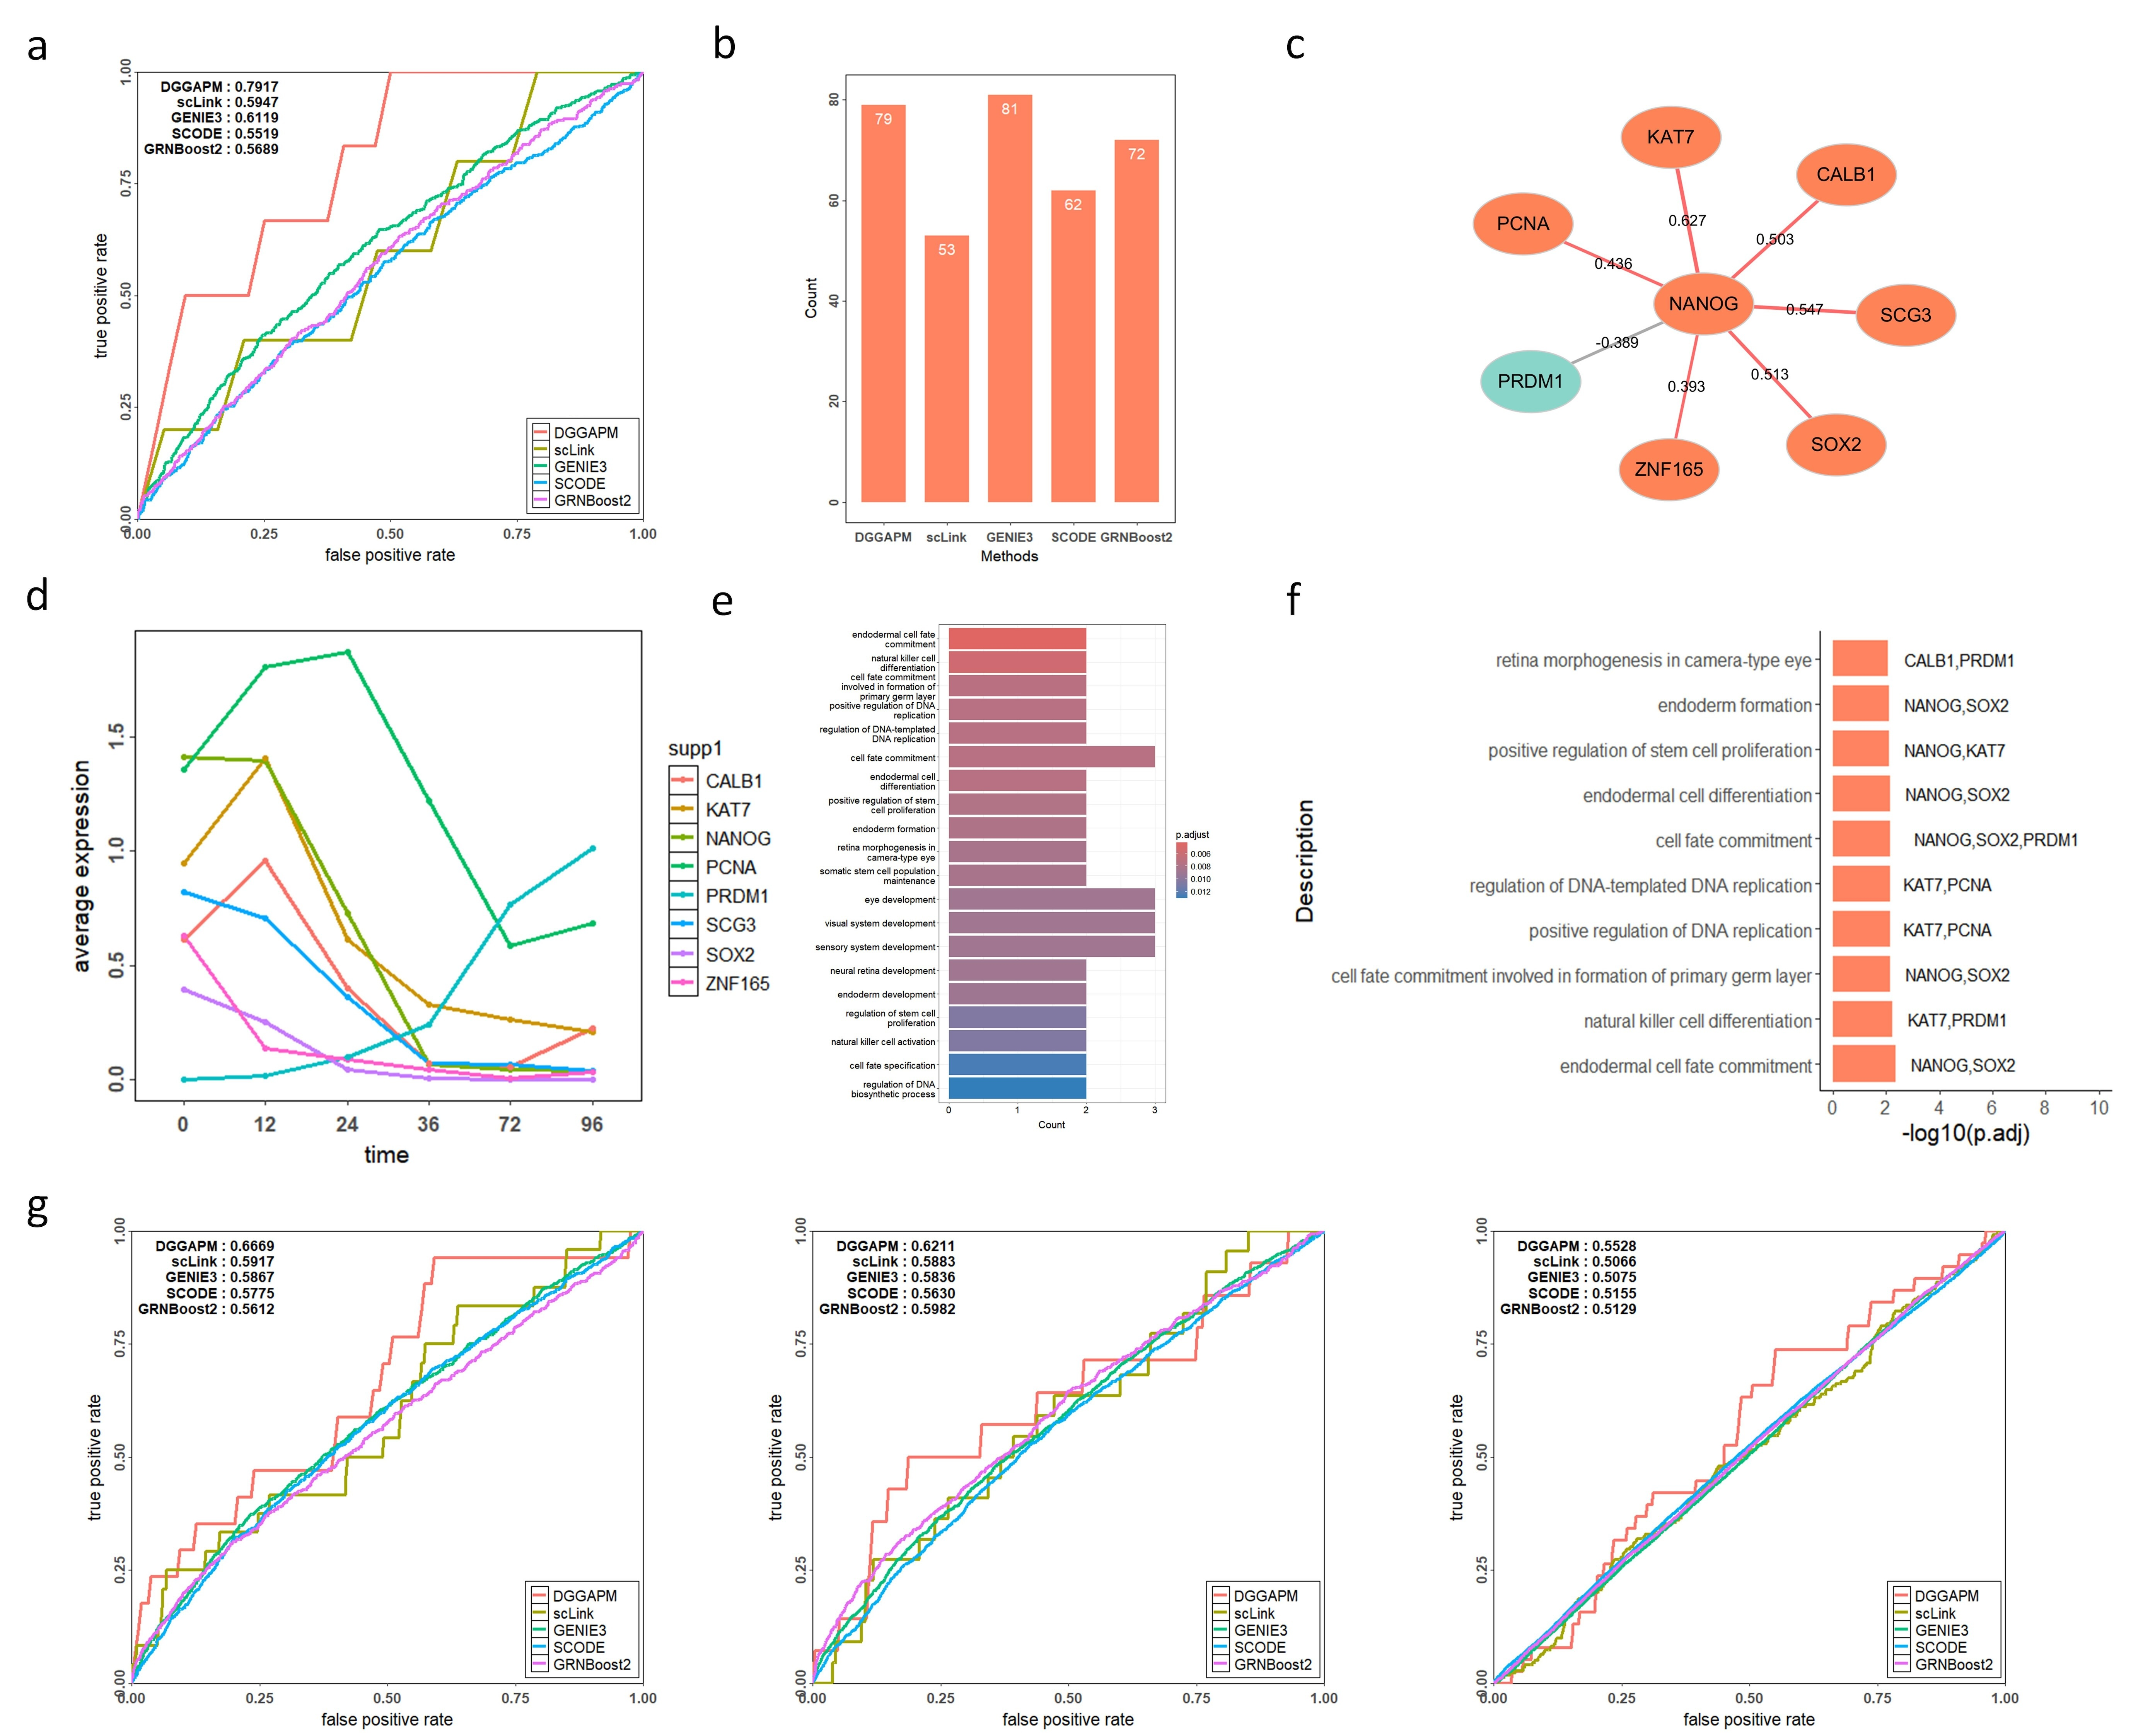
\includegraphics[width=\textwidth]{./fig/hESC2.jpeg}
	\caption{\textbf{Validation of the algorithm in human embryonic stem cells.}
	\textbf{a}, ROC curves and AUC values obtained by applying our algorithm, along with scLink, GENIE3, SCODE, and GRNBoost2 algorithms, on 714 cells and 100 genes.
	\textbf{b}, After comparison with the ground truth in the dataset, the number of correct edges identified by the five algorithms among the top 1000 edges is shown.
	\textbf{c}, The network diagram displays seven genes associated with the NANOG gene and the magnitude of their correlations. Node colors represent the categories to which the genes belong, with darker edge colors indicating stronger correlations.
	\textbf{d}, The line chart represents the average expression values of 8 genes at each time point (0, 12, 24, 36, 72, and 96 hours).
	\textbf{e}, The eight genes were analyzed for enrichment in terms of biological processes, and the top 20 pathways were selected for bar graphs.
	\textbf{f}, The bar chart displays the top ten enriched biological processes, with the y-axis representing the pathway names and the x-axis representing the size of the corrected p-values in -log10. Data labels represent the genes involved in each pathway.
	\textbf{g}, Gene expression data from different numbers of genes were selected for the experiment to evaluate the method further. Specifically, the top 200 and top 400 genes were selected among the highly variable genes sorted by their degree in the real network, and the top 400 genes were selected based on the degree of nodes in the real network.
	}
	\label{fig:hESC2}
\end{figure*}


\begin{figure*}[htb]
	\centering
	\includegraphics[width=\textwidth]{./fig/mESC1.png}
	\caption{\textbf{Identification of gene co-expression networks from mouse embryonic stem cells.}
	\textbf{a}, Correlation heatmap of $100$ genes divided into four groups in the mESCs dataset.
	\textbf{b}, After enrichment analysis of the four modules, the top $6$ pathways from each module were merged. The corrected pathway p-value is represented as -log$10$. The larger the value, the more significant the pathway, with brighter colors indicating higher significance.
	\textbf{c}, A partial gene co-expression network with genes colored according to different categories. Red edges represent positive correlations, while gray edges indicate negative correlations. Shaded areas denote submodules composed of varying gene sets.
	}
	\label{fig:s1}
\end{figure*}

\begin{figure*}[!htb]
	\centering
	\includegraphics[width=\textwidth]{./fig/mESC2.png}
	\caption{\textbf{Validation of the algorithm in mouse embryonic stem cells.}
	\textbf{a}, ROC curve and AUC analysis of $421$ cells and $100$ genes using our algorithm alongside scLink, GENIE3, SCODE, and GRNBoost2.
	\textbf{b}, Comparison with ground truth data from the dataset, showing the number of correctly identified edges among the top $100$ and $200$ predicted edges for each of the five algorithms.
	\textbf{c}, Network diagram illustrating five genes associated with Sox2 and their correlation strengths. Node colors represent the gene categories, while darker edge colors indicate stronger correlations.
	\textbf{d}, Line chart depicting the average expression levels of six genes at $0$, $12$, $24$, $48$, and $72$ hours.
	\textbf{e}, Enrichment analysis of these six genes in biological processes, with the top $20$ pathways visualized in a bar chart.
	\textbf{f}, Bar chart displaying the top $10$ enriched biological pathways. The y-axis represents pathway names, while the x-axis indicates the adjusted p-value (-log$10$ transformation). Data labels denote the number of genes involved in each pathway.
	}
	\label{fig:s2}
\end{figure*}

\begin{figure*}[!htb]
	\centering
	\includegraphics[width=\textwidth]{./fig/mHSC1.png}
	\caption{\textbf{Identification of gene co-expression networks from mouse hematopoietic stem cells. }
	\textbf{a}, Correlation heatmap of $100$ genes divided into five groups within the mHSCs dataset.
	\textbf{b}, Enrichment analysis was performed on the five modules, and the top five pathways from each module were merged. The adjusted pathway p-values are represented as -log$10$.
	\textbf{c}, A partial gene co-expression network with nodes colored according to different categories.
	}
	\label{fig:s3}
\end{figure*}


\begin{figure*}[h!]
	\centering
    \includegraphics[width=\textwidth]{./fig/mHSC2.png}
	\caption{\textbf{Validation of the algorithm in mouse hematopoietic stem cells.}
	We compared our algorithm's performance against four existing algorithms by generating receiver operating characteristic (ROC) curves and calculating the area under the curve (AUC). 
	\textbf{a} and \textbf{b}, We assessed two gene sets: the top $100$ highly variable genes with a high degree in the true network, and the top $100$ genes ranked by degree.
	After comparison with ground truth in the dataset, the correct number of edges in the first $1000$ edges was found by the four algorithms.
	\textbf{c}, We compared the number of true positive edges identified by the five algorithms within the top $100$ and $200$ edges, using the ground truth from the dataset as a reference. 
	\textbf{d}, A network graph was constructed to visualize the relationships of six genes associated with the GATA2 gene.
	\textbf{e}, Node colors represent gene categories, and edge colors indicate positive or negative correlations. Gene ontology (GO) enrichment analysis was performed on seven genes, and the top $20$ pathways were selected for a bar plot. 
	\textbf{f}, The bar plot illustrates the top $10$ enriched pathways, with the y-axis representing pathway names and the x-axis representing the -log10 of the adjusted p-values. Data labels indicate the genes involved in each pathway.
	}
	\label{fig:mHSC2}
\end{figure*}

\end{document}
